\chapter{Análisis de otras señales}
Utilizando señales (i)cuadradas, (ii)triangulares(simetría 50\%) y (iii)un tren de pulsos con $DC=33.3\%$
\begin{enumerate}
    \item Se analizó analíticamente el espectro de la señal
    \item Se simuló el espectro mediante MATLAB
    \item Se midió la señal con el analizador de espectros
    \item Se calculó el DC en función a la medición
\end{enumerate}

\section{Señal Cuadrada}
    \subsection{Análisis matemático}

    Dado que el análisis es de la señal dada en la figura \ref{fig:2,1,1}
    se observa que para un análisis de Fourier se trata de una onda
    impar:

    \begin{figure}[ht]
        \begin{center}
            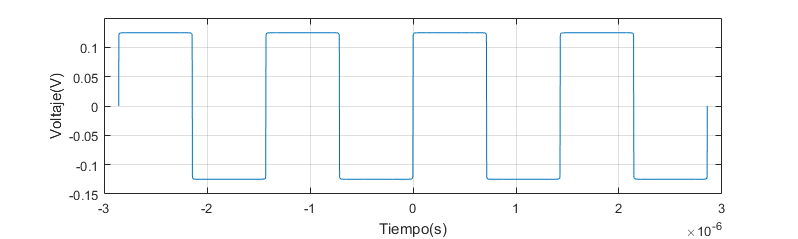
\includegraphics[width=\linewidth]{contenido/img/sig_sqr.png}
            \caption{Señal cuadrada con las características dadas}
            \label{fig:2,1,1}
        \end{center}
    \end{figure}

    Por lo tanto, la serie de Fourier estará dada por sólo senos:

    \begin{equation}
        S(t) = \sum_{k=1}^{\infty} B_{2k-1} sen(2 \pi f (2k-1) t)
    \end{equation}

    \begin{equation}
        B_{2k-1} =\frac{1}{\pi (2k-1)}
    \end{equation}

    Por lo tanto, las amplitudes observadas serán las de los armónicos
    impares de la fundamental, mientras que los armónicos pares se anulan.
    
    \subsection{Simulación del Espectro}
    Dado que se tienen las amplitudes de las diferentes frecuencias que
    conforman la señal cuadrada, se pueden calcular las potencias entregadas
    sobre la entrada del analizador, teniendo en cuenta que tiene una
    resistencia de $50\si{\ohm}$.
    Por lo tanto, el espectro observado en el analizador debería ser el visto en la figura
    \ref{fig:2,1,2}. De esta se puede observar que las potencias de los
    armónicos de mayor orden son cada vez menores.

    Debe notarse que este espectro se vería en una mitad del analizador,
    dado que las frecuencias multiplicadoras al oscilador local son sumadas
    y restadas respecto a este.

    \begin{figure}[ht]
        \begin{center}
            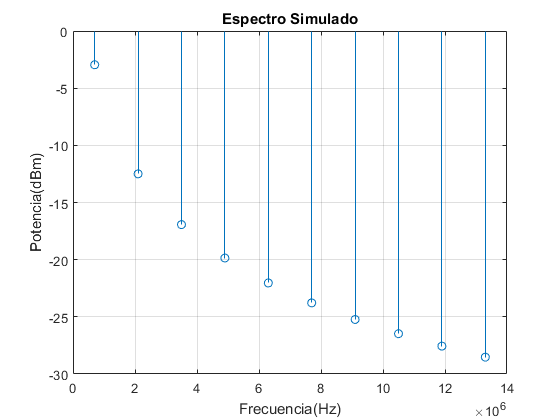
\includegraphics[width=0.75\linewidth]{contenido/img/spect_sqr.png}
            \caption{Simulación de las potencias a ser observadas}
            \label{fig:2,1,2}
        \end{center}
    \end{figure}

    \subsection{Medición en el Analizador de Espectros}

    \begin{figure}[ht]
        \begin{center}
            \caption{Pantalla del Analizador de la señal cuadrada}
            \label{fig:ansr,sqr}
        \end{center}
    \end{figure}

    \subsection{Cálculo del DC}
    Observando la salida del analizador de espectros, se pueden contar la cantidad 
    de armónicos con potencia 0 (p) y comparar esa cantidad a la cantidad total de
    armónicos que deberían verse en pantalla(q). Con estos datos, se puede utilizar
    la expresión \ref{eq:DC} para calcular el Duty Cycle.

    \begin{equation}
        DC = \frac{p}{q}
        \label{eq:DC}
    \end{equation}

    Dado que en la salida del analizador observada en la figura \ref{fig:ansr,sqr}
    se puede observar que uno de cada dos armónicos están anulados, entonces el
    Duty Cycle es de $50 \%$.

\section{Señal Triangular}
    \subsection{Análisis matemático}

    Dado que el análisis es de la señal dada en la figura \ref{fig:2,2,1}
    se observa que para un análisis de Fourier se trata de una onda
    impar:

    \begin{figure}[ht]
        \begin{center}
            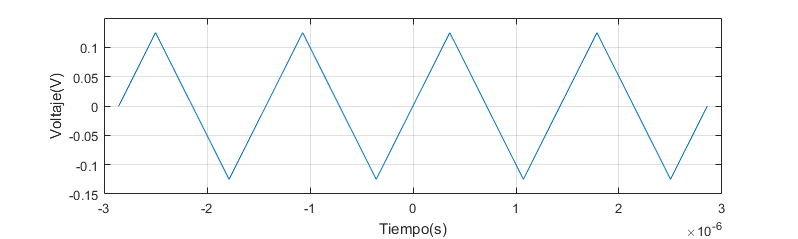
\includegraphics[width=\linewidth]{contenido/img/sig_tri.png}
            \caption{Señal cuadrada con las características dadas}
            \label{fig:2,2,1}
        \end{center}
    \end{figure}

    Por lo tanto, la serie de Fourier estará dada por sólo senos:

    \begin{equation}
        S(t) = \sum_{k=1}^{\infty} B_{2k-1} sen(2 \pi f (2k-1) t)
    \end{equation}

    \begin{equation}
        B_{2k-1} =\frac{2}{\pi^2 (2k-1)^2}
    \end{equation}

    Por lo tanto, las amplitudes observadas serán las de los armónicos
    impares de la fundamental, mientras que los armónicos pares se anulan.

    \subsection{Simulación del Espectro}
    Bajo el mismo método que en la señal cuadrada, se simuló el espectro
    de la señal triangular como se ve en la figura \ref{fig:2,2,1}. Se puede
    observar que, a diferencia de la señal cuadrada, la atenuación de cada
    armónico de mayor orden es doblemente mayor(figura \ref{fig:2,2,2}).

    \begin{figure}[ht]
        \begin{center}
            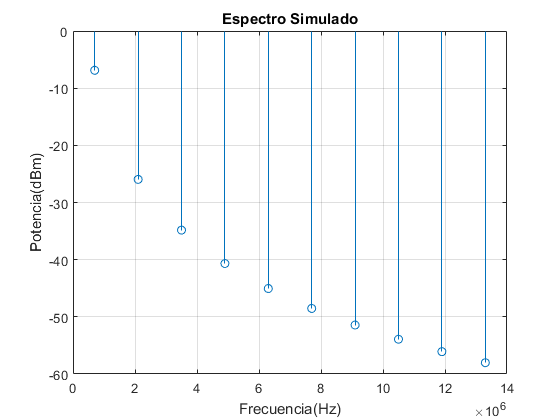
\includegraphics[width=0.7\linewidth]{contenido/img/spect_tri.png}
            \caption{Simulación de las potencias a ser observadas en la señal triangular}
            \label{fig:2,2,2}
        \end{center}
    \end{figure}

    \subsection{Medición en el Analizador de Espectros}

    \begin{figure}[ht]
        \begin{center}
            \caption{Pantalla del Analizador de la señal triangular}
            \label{fig:ansr,tri}
        \end{center}
    \end{figure}

\section{Tren de Pulsos}
    \subsection{Análisis matemático}

    Dado que el análisis es de la señal dada en la figura \ref{fig:2,3,1}
    se observa que para un análisis de Fourier se trata de una onda
    par:

    \begin{figure}[ht]
        \begin{center}
            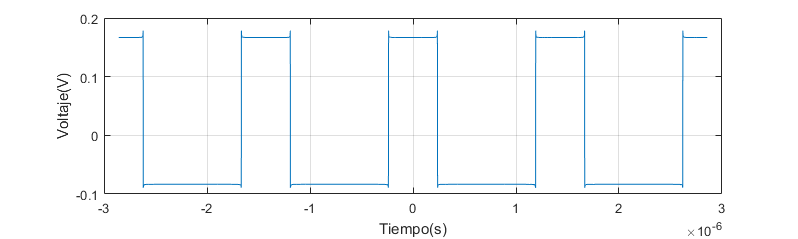
\includegraphics[width=\linewidth]{contenido/img/sig_sqr33.png}
            \caption{Señal cuadrada con DC 33.33\%}
            \label{fig:2,3,1}
        \end{center}
    \end{figure}

    Por lo tanto, la serie de Fourier estará dada por sólo senos:

    \begin{equation}
        S(t) = \sum_{n=1}^{\infty} A_{n} sen(2 \pi f n t)
        \label{eq:sqr33}
    \end{equation}

    \begin{equation}
        A_{n} =\frac{1}{\pi n} \cdot sen(\frac{\pi}{3}n)
        \label{eq:sqr33amp}
    \end{equation}

    De la expresión	\ref{eq:sqr33amp}, se puede observar que la amplitud de cada armónico
    múltiplo de 3 se verá anulado.
    
    \subsection{Simulación del Espectro}
    Se tuvieron en cuenta las mismas consideraciones para calcular las potencias de cada
    frecuencia, con las cuales se crea la figura \ref{fig:2,3,2}.

    Debe notarse que este espectro se vería en una mitad del analizador,
    dado que las frecuencias multiplicadoras al oscilador local son sumadas
    y restadas respecto a este.

    \begin{figure}[ht]
        \begin{center}
            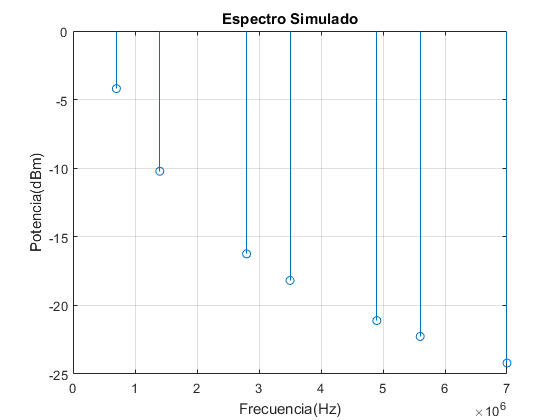
\includegraphics[width=0.75\linewidth]{contenido/img/spect_sqr33.png}
            \caption{Simulación de las potencias de la señal cuadrada con DC = 33.33\%}
            \label{fig:2,3,2}
        \end{center}
    \end{figure}

    \subsection{Medición en el Analizador de Espectros}

    \begin{figure}[ht]
        \begin{center}
            \caption{Pantalla del Analizador de la señal cuadrada}
            \label{fig:ansr,sqr33}
        \end{center}
    \end{figure}

    \subsection{Cálculo del DC}
    Utilizando nuevamente la ecuación \ref{eq:DC} se calculó, con la salida del analizador
    de espectros, el DC de la señal.

    Dado que en la salida del analizador observada en la figura \ref{fig:ansr,sqr}
    se puede observar que uno de cada tres armónicos están anulados, entonces el
    Duty Cycle es de $33.33 \%$.
\section{Conclusiones}